
\section{Resultados parciais}


%\begin{figure}[hbt!]
%    \centering
%    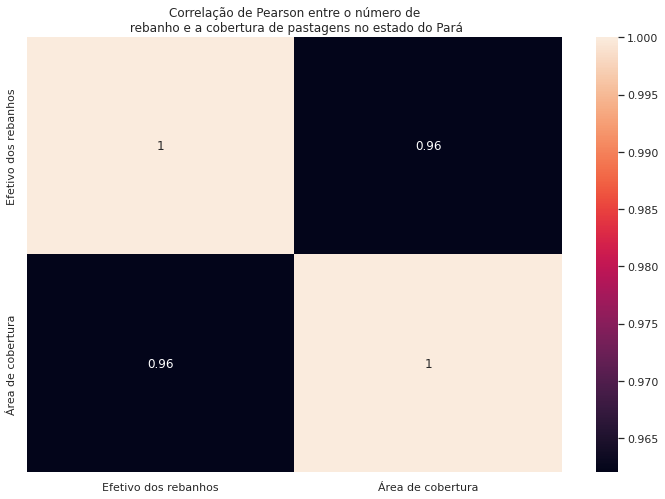
\includegraphics[width=0.7\columnwidth]{src/corr_rebanho_pastagem.png}
%    \caption{Correlação entre o número de cabeças de rebanhos em relação a área de cobertura de pastagem no estado do Pará}
%    \label{fig:corr_rebanho_pastagem}
%\end{figure}

As duas variáveis demonstraram uma alta correlação positiva, o que significa que o crescimento de uma está associada positivamente ao crescimento da outra. Para aprofundar a análise, foi gerado também um gráfico que visa entender o comportamento dos dados ao decorrer dos anos e identificar anomalias e correlações entre eles.
\begin{center}
    \begin{table}[!htb]
        \centering
        \begin{tabular}{|p{0.8\textwidth}|}
        \hline
        \textbf{Produtos das Lavouras temporárias} \\ \hline
           Abacaxi \\ 
            \hline
           Batata-doce \\ 
            \hline
           Cebola \\ 
            \hline
           Feijão \\
            \hline
           Melancia \\
            \hline
           Milho \\
            \hline
           Tomate \\
            \hline  
            \end{tabular}
        \caption{Produtos analisados das produções das lavouras temporárias}
        \label{tab:produto_analisados-lavtemp}
    \end{table}
\end{center}


\begin{center}
    \begin{table}[!htb]
        \centering
        \begin{tabular}{|p{0.8\textwidth}|}
        \hline
        \textbf{Produtos da Agropecuária} \\ 
            \hline  
            Bovino \\
            \hline  
            Bubalino \\
            \hline  
            Equino \\
            \hline  
            Caprino \\
            \hline  
            Ovino \\
            \hline  
            \end{tabular}
        \caption{Produtos analisados das produções da pecuária}
        \label{tab:produto_analisados-pecuaria}
    \end{table}
\end{center}


\newpage
\subsection{Produtos das Lavouras temporárias}

Como apresentado no gráfico abaixo, existe um crescimento visivelmente equiparado entre a cobertura da pastagem capturada pelo MapBiomas e entre o número efetivo de cabeça de rebanhos reportados pelo IBGE.

\begin{figure}[hbt!]
    \centering
    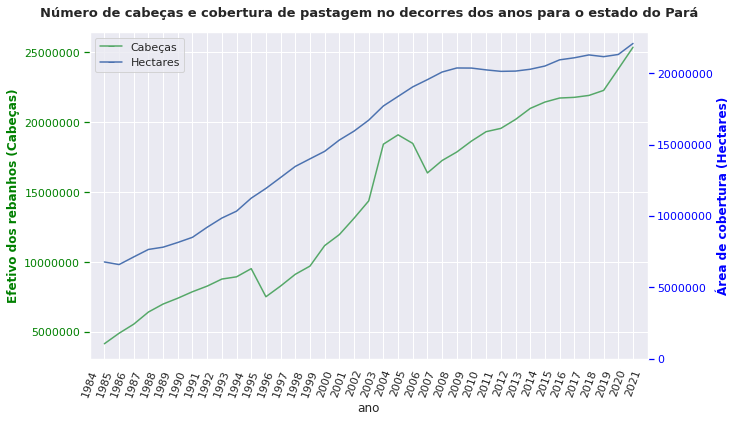
\includegraphics[width=0.6\columnwidth]{src/plots/plot-cobertura_pastagem-numero_cabecas.png}
    \centering
    \caption{Gráfico temporal de número de cabeças de rebanhos e área de cobertura de pastagem no estado do Pará}
    \label{fig:cobertura_pastagem-numero_cabeca}
\end{figure}

Para garantir a existência da correlação, foi gerado também uma análise de correlação de Pearson.

\begin{figure}[hbt!]
    \centering
    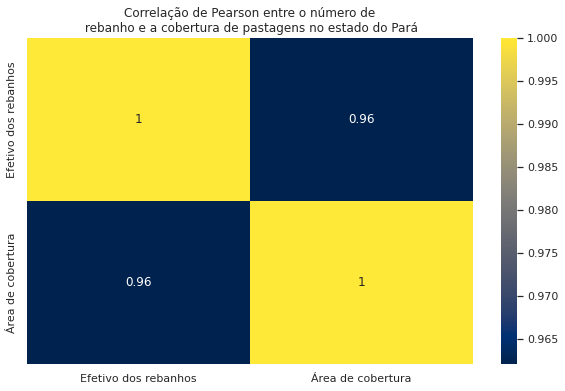
\includegraphics[width=0.6\columnwidth]{src/plots/plot_correlacao-cobertura_pastagem-numero_cabecas.png}
    \centering
    \caption{Gráfico de correlação de Pearson de número de cabeças de rebanhos e área de cobertura de pastagem no estado do Pará}
    \label{fig:correlacao-cobertura_pastagem-numero_cabecas}
\end{figure}

Foi concluído que existe uma correlação notável e relevante entre a área de cobertura da pastagem e o crescimento na produção de cabeças nos produtos pecuários no estado do Pará dos anos de 1984 até 2021.


\subsection{Produtos das lavouras temporárias}

É importante ressaltar que o produto de Soja foi removido da análise das lavouras temporárias para ser analisado separadamente. Os produtos apresentados nos gráficos são referentes aos que constam na tabela de produtos das lavouras temporárias \ref{tab:produto_analisados-lavtemp}.

Como apresentado no gráfico abaixo, existe um crescimento sutilmente visível entre a área de cobertura das lavouras temporárias e a produção dos produtos de lavouras temporárias, entretanto, é possível notar a existência de uma queda na área de cobertura no ano de 2019, porém a produção dos produtos de lavouras temporárias se mantiveram crescentes, conforme os dados reportados pelo IBGE.

\begin{figure}[hbt!]
    \centering
    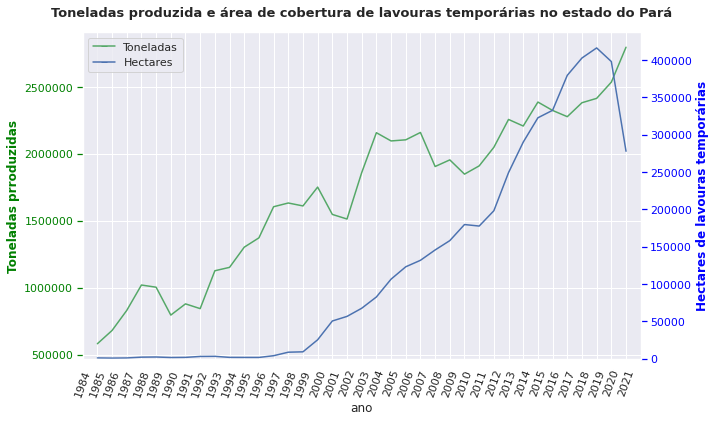
\includegraphics[width=0.6\columnwidth]{src/plots/plot-lavouras_temp.png}
    \centering
    \caption{Gráfico temporal da quantidade produzida e área de cobertura de lavouras temporárias no estado do Pará}
    \label{fig:cobertura_pastagem-numero_cabeca}
\end{figure}

Foi observado também a existência de uma alto valor no valor de correlação de Pearson, apesar da anomalia supramencionada. O valor expresso foi de 0.83, uma correlação muito relavante, indicando a existência de relação entre os valores dos dados disponibilizados pelo MapBiomas e os dados de produção de produtos de lavouras temporárias apresentados pelo IBGE

\begin{figure}[hbt!]
    \centering
    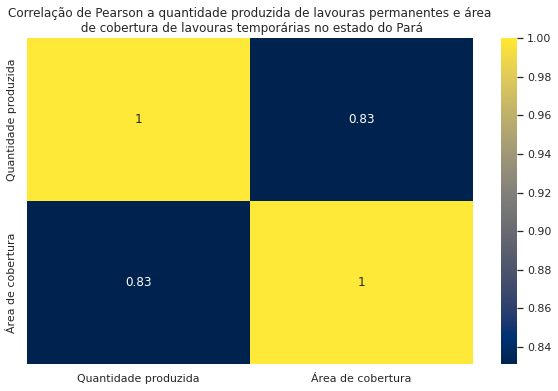
\includegraphics[width=0.6\columnwidth]{src/plots/plot_correlacao-lavouras_temp.png}
    \centering
    \caption{Gráfico de correlação de Pearson entre a quantidade produzida e área de cobertura de lavouras temporárias no estado do Pará}
    \label{fig:correlacao-cobertura_pastagem-numero_cabecas}
\end{figure}

Foi concluído que existe uma correlação notável e relevante entre a área de cobertura da lavouras temporárias e o crescimento na produção dos produtos de lavouras temporárias no estado do Pará dos anos de 1984 até 2021.




% -------------------- Soja ----------------------

\subsection{Soja}

A relação mais notável foi a apresentada pela produção da Soja. Ao analisar o produtos individualmente dos outros da classe de lavouras temporárias, foi observada uma correlação quase que perfeita entre o crescimento de produção de toneladas de sojas reportados pelo IBGE e a área de cobertura de soja reportados pelos dados do MapBiomas.


\begin{figure}[hbt!]
    \centering
    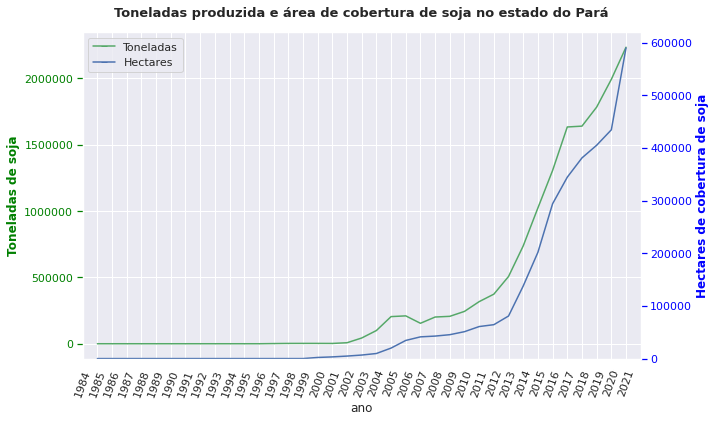
\includegraphics[width=0.6\columnwidth]{src/plots/plot-soja.png}
    \centering
    \caption{Gráfico temporal da quantidade produzida e área de cobertura de soja no estado do Pará}
    \label{fig:cobertura_pastagem-numero_cabeca}
\end{figure}

O índice de correlação de Pearson entre a área de cobertura de soja e a quantidade produzidas quase alcançou uma correlação perfeita, apresentado a correlação de 0.99, ou seja, as duas variáveis estão fortemente relacionadas.

\begin{figure}[hbt!]
    \centering
    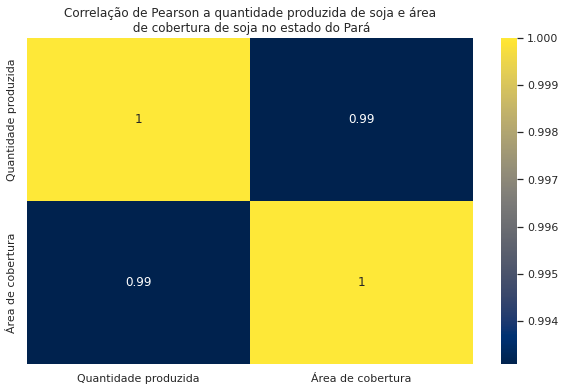
\includegraphics[width=0.6\columnwidth]{src/plots/plot_correlacao-soja.png}
    \centering
    \caption{Gráfico de correlação de Pearson entre a quantidade produzida e área de cobertura de soja no estado do Pará}
    \label{fig:correlacao-cobertura_pastagem-numero_cabecas}
\end{figure}

Foi concluído que existe uma correlação notável e extremamente relevante entre a área de cobertura do produto da soja e o crescimento na produção de soja no estado do Pará dos anos de 1984 até 2021.
